\section{Resultados}
\label{sec:resultados}

Esta seção apresenta os resultados da validação em malha aberta do
conversor VR-BESS, conduzida conforme os parâmetros descritos na
Seção~\ref{subsec:validacao_ma}: chaves $S_2$ e $S_1$ acionadas por
geradores de pulso independentes com razão cíclica fixa de $13{,}77\%$ e
$76{,}77\%$, respectivamente, comutando a $100$~kHz, sob irradiância e
temperatura constantes ($G=1000\,\text{W/m}^2$, $T=25\,^{\circ}\text{C}$).
O objetivo desta etapa não é avaliar desempenho de controle -- ainda não
implementado --, mas verificar a integração correta entre os subsistemas
de painel fotovoltaico e banco de baterias e o domínio físico do
conversor no Simscape Electrical, além de validar a razão cíclica
recalculada a partir do ponto de operação autoconsistente do arranjo
(Seção~\ref{subsec:duty_cycle}).

Na porta fotovoltaica, configurada com $N_{s,mod}=17$ e $N_{p,mod}=2$, a
corrente do arranjo ($I_{pv}$) apresentou um pico transitório de
$6{,}28$~A -- correspondente a $N_{p,mod}\times I_{SC,ref}=2\times3{,}14$~A
-- durante a energização, estabilizando-se em regime permanente em
$3{,}842$~A. A tensão do arranjo ($V_{pv}$) convergiu, com sobressinal
desprezível, para $345{,}95$~V, valor consistente com o ponto de operação
autoconsistente previsto na Seção~\ref{subsec:duty_cycle}
($V_s\approx344{,}90$~V, erro de $\approx0{,}3\%$), confirmando que a
tensão de regime do arranjo é corretamente determinada pela corrente
demandada pelo conversor, e não apenas pela associação série/paralelo
adotada.

\begin{figure}[h]
\centering
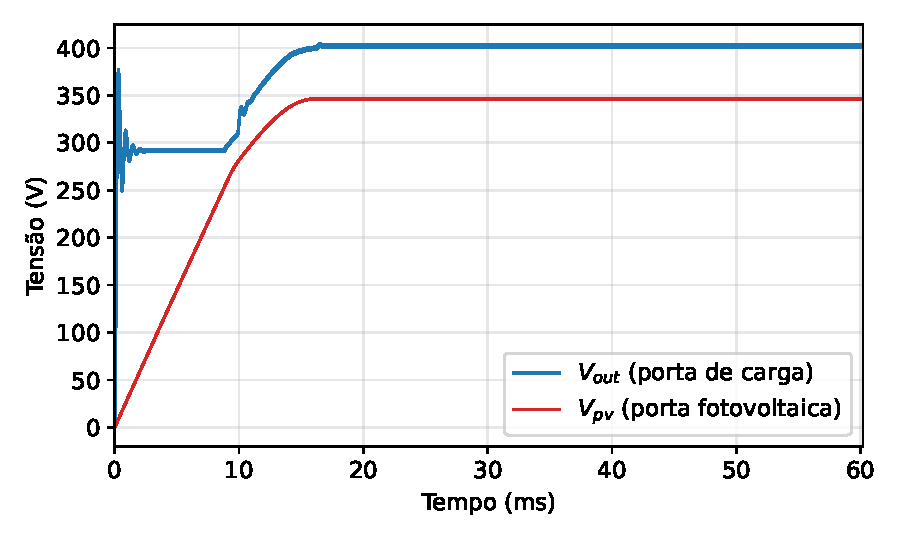
\includegraphics[width=\linewidth]{Figuras/resultado_vpv_vout.pdf}
\caption{Resposta transitória das tensões da porta fotovoltaica ($V_{pv}$)
e da porta de carga ($V_{out}$) sob comutação em malha aberta.}
\label{fig:resultado_vpv_vout}
\end{figure}

Na porta de saída, a tensão sobre a carga ($V_{out}$) convergiu, com pico
de $404{,}24$~V em $t\approx16{,}5$~ms (sobressinal de apenas
$\approx0{,}65\%$ em relação ao valor de regime), para
$401{,}62$~V, com ripple de comutação de $2{,}50$~V pico-a-pico
($\approx0{,}62\%$). Esse resultado corresponde a um desvio de apenas
$\approx0{,}4\%$ em relação à tensão de projeto de $400$~V, validando a
razão cíclica recalculada a partir do ponto de operação autoconsistente do
arranjo (Seção~\ref{subsec:duty_cycle}), em contraste com o desvio muito
maior obtido ao se utilizar a razão cíclica calculada a partir da tensão
de máxima potência nominal do arranjo (Seção~\ref{subsec:duty_cycle}). A
relação ideal de ganho do estágio Boost também se confirma:
$V_o=V_{pv}/(1-D_i)=345{,}95/0{,}8623\approx401{,}2$~V, contra os
$401{,}62$~V medidos (erro de $\approx0{,}1\%$). A corrente de carga
($I_{out}$) se estabeleceu em $2{,}510$~A, resultando em
$R_o=V_{out}/I_{out}\approx160{,}0\,\Omega$, consistente com o valor
resistivo adotado.

Na porta de armazenamento, configurada com $N_{s,bat}=15$, $N_{p,bat}=1$ e
estado de carga inicial $SOC_0=50\%$, a tensão de bateria ($V_{bat}$)
manteve-se praticamente constante em $251{,}92$~V, compatível com a tensão
em circuito aberto esperada para o arranjo
($N_{s,bat}\times E_0=15\times16{,}8=252$~V) na vizinhança de
$SOC=50\%$. A corrente de bateria ($I_{bat}$) apresentou um transitório
inicial de até $5{,}48$~A antes de se estabilizar em um valor médio de
regime de $\approx-1{,}23$~A -- negativo, na convenção positiva para
descarga adotada na Eq.~\eqref{eq:battery_terminal}, indicando
carregamento --, com ripple de comutação de $\approx0{,}037$~A
pico-a-pico. Esse valor situa-se $\approx7\%$ acima do limiar de
$0{,}5\text{C}$ ($1{,}15$~A) adotado para a corrente de carregamento,
consistente com a natureza do limitador proporcional implementado no
modelo da bateria (Seção~\ref{subsec:modelagem_bat_impl}), que permite à
corrente de regime assentar próxima ao limiar nominal sem impor um corte
abrupto. O estado de carga (SOC) permaneceu praticamente inalterado
($50{,}0004\%$) no intervalo analisado, compatível com a baixa taxa de
carregamento frente à capacidade do banco.

\begin{figure}[h]
\centering
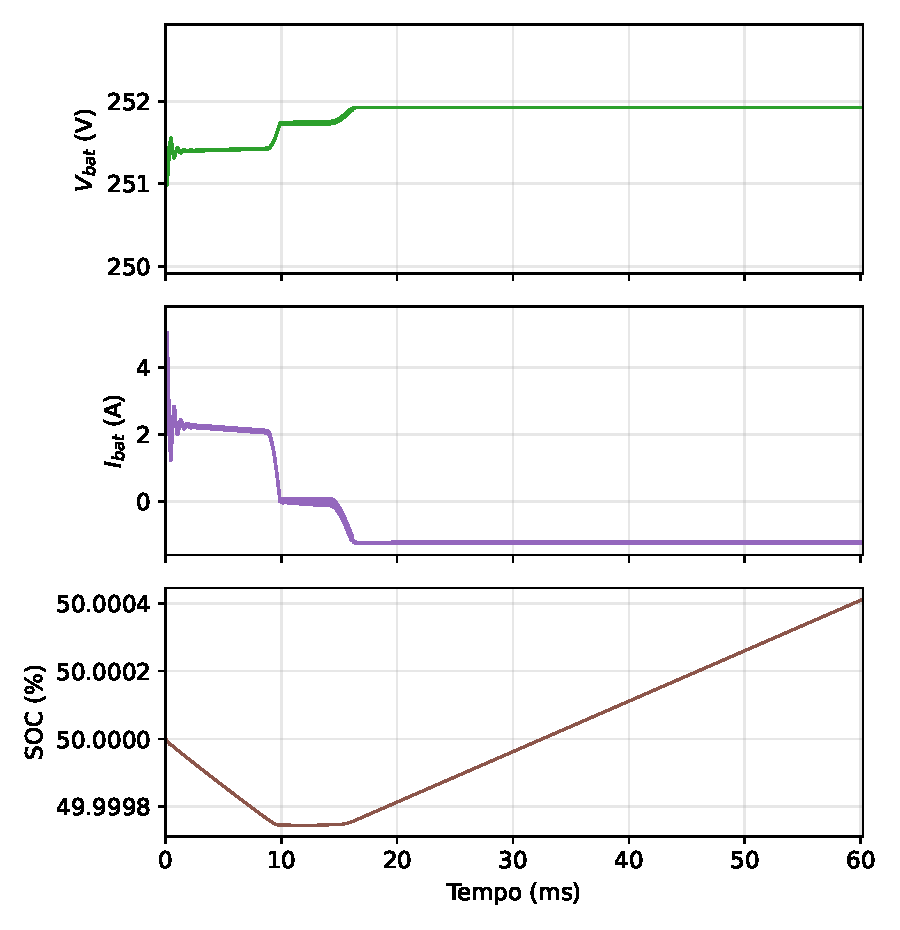
\includegraphics[width=\linewidth]{Figuras/resultado_bateria.pdf}
\caption{Tensão de bateria ($V_{bat}$), corrente de bateria ($I_{bat}$) e
estado de carga (SOC) da porta de armazenamento.}
\label{fig:resultado_bateria}
\end{figure}

Por fim, a corrente no indutor compartilhado da porta fotovoltaica
($I_s$), medida diretamente no ramo comutado, acompanhou a corrente do
arranjo $I_{pv}$ em regime ($\approx3{,}842$~A, ripple de $0{,}125$~A
pico-a-pico), com uma excursão transitória negativa de até $-0{,}60$~A
durante a energização do conversor, compatível com o comportamento
esperado de um indutor submetido a comutação dura em malha aberta.

Em conjunto, esses resultados confirmam a integração correta entre os
blocos mascarados de painel fotovoltaico e banco de baterias e o domínio
físico do conversor VR-BESS, com a tensão de saída convergindo para
próximo do valor de projeto ($401{,}62$~V frente aos $400$~V especificados)
a partir da razão cíclica recalculada pelo método de ponto fixo
apresentado na Seção~\ref{subsec:duty_cycle}. Essa validação confirma que,
diferentemente da tensão de bateria -- fixada essencialmente pela
associação série do banco --, a tensão do arranjo fotovoltaico em regime é
determinada pela corrente demandada pelo conversor, exigindo o cálculo da
razão cíclica a partir do ponto de operação autoconsistente do arranjo, e
não da tensão de máxima potência nominal. Essa validação em malha aberta
estabelece a base de simulação sobre a qual o controlador FCS-MPC,
apresentado na Seção~\ref{subsec:fcsmpc}, será implementado e avaliado --
em substituição aos geradores de pulso de razão cíclica fixa por uma lei
de comutação em tempo real capaz de manter $V_{out}$ regulado mesmo
quando a corrente de carregamento da bateria variar em relação ao ponto
de operação aqui calibrado -- na etapa subsequente deste trabalho.
